\documentclass[a4paper]{book}

% Load the VUB theme from https://gitlab.com/rubdos/texlive-vub
\usepackage{vub}

% hyperref package makes links clickable (e.g. references)
% The color is set to black for each link type
\usepackage{hyperref}
\hypersetup{
    colorlinks,
    citecolor=black,
    filecolor=black,
    linkcolor=black,
    urlcolor=black
}

% Used for abbrivations etc
\usepackage{glossaries}

% We use cleveref for better referencing control
\usepackage{cleveref}
\usepackage[natbib,style=apa]{biblatex}
\addbibresource{../bibliography.bib}

% Init glossary
\makenoidxglossaries

% Add glossary entries
% Add glossary entries
% ref glossary with \Gls{latex}
% ref acronym with \acrshort{bci} or \acrlong{bci}
\newglossaryentry{latex}
{
    name=latex,
    description={Is a markup language specially suited 
    for scientific documents}
}

%% ------- BCI related
\newacronym[plural=BCIs,firstplural=brain-computer interfaces (BCIs)]{bci}{BCI}{brain-computer interface}
\newacronym[plural=BMIs,firstplural=brain-machine interfaces (BMIs)]{bmi}{BMI}{brain-machine interface}
\newacronym[plural=BMIs,firstplural=human-machine interfaces (HMIs)]{hmi}{HMI}{human-machine interface}
\newacronym{bc}{biosignal control}{biological signal control}

\newacronym[plural=topomaps,firstplural=topographic maps (topomaps)]{topomap}{topomap}{topographic map}

\newacronym{cad}{CADx}{computer-aided diagnosis}
\newacronym{cade}{CADe}{computer-aided detection}
\newacronym{bt}{BT}{Bluetooth}
\newacronym{ac}{AC}{alternating current}

\newacronym{pca}{PCA}{principal component analysis}
\newacronym{ica}{ICA}{independent component analysis}

\newacronym[plural=CSPs, firstplural=common spatial patterns]{csp}{CSP}{common spatial pattern}
\newacronym{fbcsp}{FBCSP}{filter bank common spatial pattern}
\newacronym{pfbcsp}{PFBCSP}{penalized frequency band common spatial pattern}
\newacronym{ptfbcsp}{PTFBCSP}{penalized time-frequency band common spatial pattern}

%% ------- Medical
\newacronym{als}{ALS}{amyotrophic lateral sclerosis}
\newacronym{dmd}{DMD}{duchenne muscular dystrophy}
\newacronym{tl}{TL}{transfer learning}

\newacronym{af}{AF}{atrial fibrillation}

\newacronym{poc}{POC}{proof of concept}
\newacronym{fda}{FDA}{Food and Drug Administration}

\newacronym{ux}{UX}{user experience}
\newacronym{ui}{UI}{user interface}
\newacronym{cns}{CNS}{central nervous system}


\newacronym{lis}{LIS}{locked-in syndrome}

%% ------- Signal related

\newacronym[plural=EPs,firstplural=evoked potentials (EPs)]{ep}{EP}{evoked potential}
\newacronym[plural=ERPs,firstplural=event-related potentials (ERPs)]{erp}{ERP}{event-related potential}
\newacronym[plural=SSEPs,firstplural=steady state evoked potentials (SSEPs)]{ssep}{SSEP}{steady state evoked potential}
\newacronym{ssaep}{SSAEP}{steady-state auditory evoked potential}

\newacronym{ern}{ERN}{error-related negativity}
\newacronym{mrcp}{MRCP}{movement-related cortical potential}

\newacronym{ssvep}{SSVEP}{steady-state visual evoked potential}
\newacronym{sssep}{SSSEP}{steady-state somatosensory evoked potential}
\newacronym{aep}{AEP}{auditory evoked potential}
\newacronym{vep}{VEP}{visual evoked potential}
\newacronym{somsep}{SSEP}{somatosensory evoked potential}
\newacronym{mi}{MI}{motor imagery}
\newacronym{snr}{SNR}{signal-to-noise ratio}
\newacronym{erd}{ERD}{event-related desynchronization}
\newacronym{ers}{ERS}{event-related synchronization}


\newacronym[plural=biosignals,firstplural=biomedical signals (biosignals)]{biosignal}{biosignal}{biomedical signal}
\newacronym[plural=bioelectrical signals,firstplural=electrical biomedical signals (bioelectrical signals)]{elecbiosignal}{bioelectrical signals}{electrical biomedical signals}

\newacronym{hz}{Hz}{hertz}
\newacronym{fir}{FIR}{finite impulse response}
\newacronym{iir}{IIR}{infinite impulse response}

\newacronym{csf}{CSF}{cerebrospinal fluid}

\newacronym{eeg}{EEG}{electroencephalography}
\newacronym{ecog}{ECoG}{electrocorticography}
\newacronym{ecg}{ECG}{electrocardiography}
\newacronym{eog}{EOG}{electrooculography}
\newacronym{erg}{ERG}{electroretinography}
\newacronym{egg}{EGG}{electrogastrogram}
\newacronym{eda}{EDA}{electrodermal activity}
\newacronym{gsr}{GSR}{galvanic skin response}
\newacronym{fnirs}{fNIRS}{functional near-infrared spectroscopy}
\newacronym{ftcd}{fTCD}{functional transcranial doppler}

\newacronym{pet}{PET}{positron emission tomography}
\newacronym{spect}{SPECT}{single-photon emission computerized tomography}
\newacronym{ct}{CT}{computerised tomography}


\newacronym{deeg}{DEEG}{digital electroencephalography}
\newacronym{emg}{EMG}{electromyography}
\newacronym{meg}{MEG}{magnetoencephalography }
\newacronym{mv}{$\mu V$}{microvolts}
\newacronym{milv}{mv}{millivolts}

\newacronym{mri}{MRI}{magnetic resonance imaging}

\newacronym{fn}{FN}{false negative}
\newacronym{fp}{FP}{false positive}

\newacronym{hu}{HU}{Hounsfield unit}

%% ------- AI related
\newacronym{ai}{AI}{artificial intelligence}
\newacronym{ml}{ML}{machine learning}
\newacronym{rl}{RL}{reinforcement learning}
\newacronym{nlp}{NLP}{natural language processing}

\newacronym{sklearn}{sklearn}{scikit-learn}

\newacronym{lr}{LR}{logistic regression}
\newacronym{lda}{LDA}{linear discriminant analysis}
\newacronym{svm}{SVM}{support vector machines}
\newacronym{svc}{SVC}{C-support vector classification}
\newacronym{rbf}{RBF}{radial basis function}
\newacronym{rf}{RF}{random forest}
\newacronym[plural=ANNs,firstplural=artificial neural networks (ANNs)]{ann}{ANN}{artificial neural network}
\newacronym{nn}{NN}{neural network}
\newacronym{bpnn}{BPNN}{back propagation neural network}
\newacronym[plural=RNNs,firstplural=recurrent neural networks (RNNs)]{rnn}{RNN}{recurrent neural network}
\newacronym[plural=LSTMs,firstplural=long short-term memory networks (LSTMs)]{lstm}{LSTM}{long short-term memory network}

\newacronym{dl}{DL}{deep learning}

\newacronym{esi}{ESI}{scout EEG source imaging}

\newacronym{gan}{GAN}{generative adversarial network}
\newacronym{automl}{AutoML}{automated machine learning}

\newacronym[plural=CNNs,firstplural=convolutional neural networks (CNNs)]{cnn}{CNN}{convolutional neural network}

%% ------- AR/VR

\newacronym{vr}{VR}{virtual reality}
\newacronym{ar}{AR}{augmented reality}

% ------- Hardware
\newacronym[plural=CPUs,firstplural=central processing units]{cpu}{CPU}{central processing unit}
\newacronym[plural=GPUs,firstplural=graphics processing units (GPUs)]{gpu}{GPU}{graphics processing unit}

\newacronym{dsp}{DSP}{digitial signal processor}
\newacronym{fpga}{FPGA}{field programmable gate arrays}

\newacronym{baiid}{BAIID}{breath alcohol ignition interlock device}


% ------- Organisations
\newacronym{bbci}{BBCI}{Berlin Brain-Computer Interface research program}
\newacronym{eu}{EU}{European Union}
\newacronym{tos}{ToS}{terms of service}

% ------- Laws
\newacronym{gdpr}{GDPR}{general data protection regulation}


% ------- Metrics
\newacronym{roc}{ROC curve}{receiver operating characteristic curve}
\newacronym{auc}{AUC}{area under the (ROC) curve}


% ------- Feature extraction
\newacronym{mav}{MAV}{mean absolute value}
\newacronym{zc}{ZC}{zero crossing}
\newacronym{ssc}{SSC}{slope sign changes}
\newacronym{wl}{WL}{waveform length}
\newacronym{pe}{PE}{permutation entropy}
\newacronym{apen}{ApEn}{approximate entropy}
\newacronym{fuzzen}{FuzzEn}{fuzzy entropy}
\newacronym{ft}{FT}{Fourier transform}
\newacronym{ift}{IFT}{inverse Fourier transform}
\newacronym{dft}{DFT}{discrete Fourier transform}
\newacronym{idft}{IDFT}{inverse discrete Fourier transform}
\newacronym{fft}{FFT}{fast Fourier transform}

\newacronym{psd}{PSD}{power spectral density}
\newacronym{iwmf}{IWMF}{intensity weighted mean frequency}
\newacronym{iwbw}{IWBW}{intensity weighted bandwidth}

\newacronym{stft}{STFT}{short-time Fourier transform}
\newacronym{wt}{WT}{wavelet transformation}




% English title
% TODO:
%   - Correct Title and Subtitle
% ----------  
% Questions:
%   - Is date correct as just year
%   - Is it indeed so that the title of my education should stay in dutch?
%   - Layout ok?

\title{Brain controlled what?}
\pretitle{\flushleft{Master thesis submitted in partial fulfilment of the requirements for the degree of Master of Science in de Ingenieurswetenschappen: Computerwetenschappen}}
\subtitle{A computer scientist's guide to brain-computer interfaces and a comparison study of multiple state-of-the-art motor imagery EEG classification approaches}
\author{Lennert Bontinck}
\date{2021 - 2022}
\promotors{Promotors: Prof. Dr. Geraint Wiggins \& Prof. Dr. Kevin De Pauw}
\advisors{Advisor: Arnau Dillen}
\faculty{Faculty of Sciences and Bioeengineering Sciences}
\begin{document}
\frontmatter
\maketitle

% Dutch title
\pretitle{\flushleft{Proefschrift ingediend met het oog op het behalen van de graad van Master of Science in de Ingenieurswetenschappen: Computerwetenschappen}}
\title{Evaluatie en uitbreiding van decoderings- methoden voor ingebeelde motorische handelingen}
\subtitle{Inleiding tot hersen-computerkoppelingen en de effecten van toegevoegde LSTM lagen in CNN-classificatiemethoden}
\date{2021 - 2022}
\promotors{Promotors: Prof. Dr. Geraint Wiggins \& Prof. Dr. Kevin De Pauw}
\advisors{Copromotor : Arnau Dillen}
\faculty{Faculteit Wetenschappen en Bio-ingenieurswetenschappen}
\maketitle

% Abstract
\glsresetall

\chapter*{Abstract}
\label{ch:abstract}

\Glspl{bci} are systems that aim to translate brain signals into actions.
A recent rise in both scientific and commercial interest in these systems has helped popularize them outside highly specialized labs.
However, the highly interdisciplinary nature of \gls{bci} research among many other complex factors results in a steep learning curve which deters many individuals who wish to work with these kinds of systems.

This master thesis aims to facilitate this entry into the \gls{bci} field for computer scientists.
Through an extensive but intuitive introduction of \glspl{bci}, a scoping review is performed to address recent advancements, current opportunities and open issues in the field together with some ethical concerns.
This intuitive understanding is then grounded by providing the required technical background on the \glspl{biosignal}, brain signal acquisition systems and the general \gls{mi} \gls{eeg} classification pipeline that enables these systems.

This theory is put to practice by discussing, implementing and evaluating seven unique offline \gls{mi} \gls{eeg} classification pipelines.
In particular, two traditional two-step \gls{ml} approaches based on \gls{csp} feature extraction, three literature proposed state-of-the-art \gls{cnn} based approaches and two proposed extensions providing \gls{lstm} functionalities to such \gls{cnn} models are considered.
The latter extensions were proposed to explore the question if added \gls{lstm} functionalities helps the state-of-the-art EEGNet model in optimally decoding \gls{mi} \gls{eeg} data.
It was found that for 1.5-second windowed samples centred around a known event, one of the \gls{lstm} extension outperforms the \gls{cnn} based state-of-the-art EEGNet model it is based on in an intersubject evaluation strategy for testing three-class \gls{mi} \gls{eeg} classification performance.
This model obtained a mean test accuracy of  $65.52$ ± $0.89$, over the $60.68$ ± $1.64$ obtained by the EEGNet model it is based on.
Other \gls{cm} derived metrics were also found favourable for the extension.
It is discussed how this difference could increase further when using a different windowing technique.

Due to the considerable amount of information this master thesis wishes to provide, a multitude of new questions and potential future work arises.
Some of these discussed future possibilities, such as moving from the offline \gls{mi} \gls{eeg} classification pipelines to a complete \gls{bci} system, benefit from pilot studies also presented in this master thesis.
In this regard, a pilot study found that an intersubject test accuracy of over 90\% can be reached for certain subjects of the open-source dataset used.
% TODO:
%   - 
% ----------  
% Questions:
%   - Should this be included in ToC?
%   - Is inspiration for text an issue?

\chapter{Acknowledgements}
\label{ch:acknowledgements}

% NOTE: textual inspiration from: https://esl.gatech.edu/sites/default/files/LI/li-how_to_write_acknowledgements_in_a_dissertation.pdf
I'm extremely grateful to both my supervisor Prof. Dr. Geraint Wiggins and advisor Mr. Arnau Dillen for allowing me to write this thesis with a subject tailored to my interests.
This thesis would not have been possible without their helpful advise, constructive criticism and insightful suggestions.
Their patients cannot be underestimated and the organised biweekly meetings were simply invaluable.
I must also thank Prof. Dr. Jef Vandemeulebroucke for teaching both the biomedical signals and imaging course as well as the clinical decision support systems course.
The contents of these courses has contributed to a better understanding on some of the physical phenomena and used technologies addressed in this thesis.
I’d also like to recognize the statistical and writing expertise gained through the methods of scientific research course by Prof. Dr. Bart de Boer.
Lastly, I gratefully acknowledge the unparalleled support of my girlfriend, parents and friends throughout the sometimes stressful process of this master thesis.

% TODO
Todo: complete with additional people if need be.

% ToC
\tableofcontents
\mainmatter

% Main content
% TODO:
%   - References in section helping people with disabilities for examples
%   - More complete and referenced 1.1
%   - Longer more descriptive titles
% ----------  
% Questions:
%   - Should we also use parts or not?

% Uncomment this if use of parts is desired
%\part{First part}

\chapter{Introduction}
\label{ch:introduction}

\Glspl{bci} and \glspl{bmi} are starting to gather more interest from the general public.
These systems, consisting of hardware and software, aim to read and stimulate a user's biomedical signals for a wide range of purposes.
Neuralink, an Elon Musk company, helped to popularize them outside of the research field.
Neuralink's initial white paper discusses its aim to create a scalable high-bandwidth \acrshort{bmi} system, focusing on its mechanical achievements \citep{neuralink_whitepaper}.
Only a mere year later, the company held a conference with a live demo of their \acrshort{bmi} implanted into the skulls of pigs.

Whilst such novel interaction application have yet to see wide spread market adoption, \acrshortpl{bci} have been studied for decennia by researchers such as \citet{early_bci}.
An in-depth history from \acrshortpl{bci} can be found from Andrea \citet{bci_history}.
\citet{bci_review} gives an overview of the different kinds of \acrshortpl{bci} and corresponding techniques to be used.
These sources give a great high-level insight into the technology and terminology used in this field.
A good introductory book on \acrshortpl{bci} from this same period is one from the well-known Professor in this field: Jonathan Wolpaw \citep{bci_book}.

Whilst techniques used today remain relatively similar to those discussed in these older sources, the hardware complexity has been evolving drastically.
An important issue researchers keep getting confronted with is the fact that there's still a lot of mysteries about the brain's inner working, leaving many of the finer intercepted brain signals unexplained.
\citet{brainmapping} states that the progress of mapping the brain and it's billions of sensors and connections is accelerating yet still far from finished.
This mapping would be a huge step in understanding the brain.

Luckily, novel \gls{ml} techniques can help with processing and reasoning on the data these systems collect.
Especially due to recent developments in \gls{dl} and \gls{nn}, \acrshortpl{bci} are being used more in treating neurological diseases \citep{bci_diseases} but also more commercial applications, like a brain-controlled "virtual keyboard" as discussed by \citet{bci_keyboard}.

A challenge with \acrshort{dl} applications in general, and certainly with \acrshortpl{bci}, is the fact that training a deep learner in an unsupervised manner can take a lot of data and time and be unpredictable due to it's black box principle.
These things are unwished-for in \acrshort{bci} systems, especially when not only reading but also stimulating brain signals.
In general, full supervised learning isn't possible either due to the lack of understanding the brain signals.
Therefore, low-confidence labeled data is often used in a semi-supervised fashion as explained by \citet{deep_learn_low_label}.

\section{Gaining popularity}
\label{sec:introduction_gaining_popularity}

As was already discussed, Neuralink, a company by Elon Musk aiming to provide an invasive \acrshort{bci} to be used by the masses as a mean for fast communication between human and machine, has put the research field in new daylight.
However, the reason \acrshortpl{bci} applications are gaining more and more interest follows from a wide variety of reasons.
The following section will discuss the most important ones.

\subsection{Commercialisation by big tech}
\label{subsec:introduction_gaining_popularity_big_tech}
TODO

\subsection{Improved machine learning}
\label{subsec:introduction_gaining_popularity_improved_ml}
TODO

\subsection{More affordable hardware}
\label{subsec:introduction_gaining_popularity_affordability}
TODO

\subsection{Boost in efficiency}
\label{subsec:introduction_gaining_popularity_efficiency}
TODO

\section{Helping people with disabilities}
\label{sec:introduction_helping_disabled}

Whilst the commercial interest of \acrshortpl{bci} is apparent, it is not the only reason these systems are gaining popularity.
As technology evolves, it has often been the case that people with certain disabilities benefit from the evolution as well.
Recently, image and speech to text technology has found its way directly into smartphone operating systems.
Whilst it is handy for most to have the capability of generating subtitles for an audio track playing on your phone, people with limited hearing now have a direct way to enjoy more content too.
Those people who have difficulties with vision can benefit greatly from a camera app with scene detection and text detection.
But even simple application such as a color picker on the camera can aid people who have color blindness in determining whether if a banana is ripe and more.
This section will highlight some of the benefits \acrshortpl{bci} can offer to people with disabilities.

\subsection{Parkinson's disease}
\label{subsec:introduction_helping_disabled_parkinson}
TODO

\subsection{Audiovisual aid}
\label{subsec:introduction_helping_disabled_audiovisual}
TODO

\subsection{Wheelchair users}
\label{subsec:introduction_helping_disabled_wheelchair}
TODO

\section{Small projects with big impact}
\label{sec:introduction_small_projects}
TODO

\subsection{TODO: example small project}
\label{subsec:introduction_small_projects_XXX}
TODO

\subsection{TODO: example small project}
\label{subsec:introduction_small_projects_YYY}
TODO

\subsection{Using a 3 signal system for basic controls}
\label{subsec:introduction_small_projects_ours}
TODO

\section{Ethical questions}
\label{sec:introduction_ethical}
TODO

\subsection{Risk of data mining for advertising}
\label{subsec:introduction_ethical_ads}
TODO

\subsection{Making the rich even richer}
\label{subsec:introduction_ethical_expensive}
TODO

\subsection{Confronting users with their brain}
\label{subsec:introduction_ethical_medical_users}
TODO
% TODO:
%   - Make this background chapter
%   - Section on ethics
%   - Split out your own work from literature
%   - Move BCI pipeline to separate chapter
% ----------  
% Questions:
%   - XXX

% https://www.brainlatam.com/blog/wet-dry-active-and-passive-electrodes.-what-are-they-and-what-to-choose-413
% https://www.brainlatam.com/blog/a-brief-introduction-to-eeg-and-the-types-of-electrodes-75

% Goed boek voor sources bci_review_book_chapter

% In a new chapter, reset the GLS to once again use full version in first occurence
\glsresetall

\chapter{Biomedical signals}
\label{ch:biomedical_signals}

% ---------------------------------------------- 

\section{Better understanding the data used by BCIs}
\label{sec:biomedical_signals_why}

% TODO
\lipsum[1-2]

% ---------------------------------------------- 

\section{Origin of brain-signals}
\label{sec:biomedical_signals_origin}

% TODO
\lipsum[1-2]

% - - - - - - - - - -

\subsection{Bioelectricity in the human body}
\label{subsec:biomedical_signals_origin_bioelectricity}

% TODO
\lipsum[1-4]

% - - - - - - - - - -

\subsection{Measurable brain activity}
\label{subsec:biomedical_signals_origin_brain_activity}

% TODO
\lipsum[1-3]


% - - - - - - - - - -

\subsection{Anatomy of the brain}
\label{subsec:biomedical_signals_origin_anatomy_brain}

% TODO
\lipsum[1-4]

% - - - - - - - - - -

\subsection{Neuroplasticity and inter-human variation}
\label{subsec:biomedical_signals_origin_general_brain_layout}

% TODO
\lipsum[1-3]

% ---------------------------------------------- 

\section{Types of brain-signals}
\label{sec:biomedical_signals_type_of_signals}

% TODO
\lipsum[1-2]

% - - - - - - - - - -

\subsection{Brain waves frequencies}
\label{subsec:biomedical_signals_type_of_signals_brain_wave}

% TODO
\lipsum[1-2]

% - - - - - - - - - -

\subsection{Event related potentials}
\label{subsec:biomedical_signals_type_of_signals_erp}

% TODO
% P300 en andere signalen vermeld in introduction
\lipsum[1-2]

% - - - - - - - - - -

\subsection{Motor imagery}
\label{subsec:biomedical_signals_type_of_signals_motor_imagery}

% TODO zie chapter 23 bci_handbook
% Issues MI: https://www.frontiersin.org/articles/10.3389/fnins.2021.824759/full
\Gls{mi} is the process in which a person generates brain-activity in the motor cortex merely by imagining motor movements.
\Gls{mi}-based \glspl{bci} are interesting because they don't require any external stimulus nor effective motor movements

\lipsum[1-3]

% ---------------------------------------------- 


\section{Measuring brain-signals}
\label{sec:biomedical_signals_measuring}

% TODO
\lipsum[1-2]

% ---------------------------------------------- 

\subsection{Measuring modalities}
\label{subsec:biomedical_signals_measuring_modalities}
% EEG ECOG ETC ETC

% TODO
\lipsum[1-5]

Research by \citet{human_eeg_discovery} is the first in describing the measurement of brain waves from the human skull in a non-invasive manner.
Because of this, the German neuroscientist and psychiatrist Hans Berger is often seen as the inventor of \gls{eeg}.
Whilst he was one of the first to use the term \textit{elektrenkephalogramm}, it was Richard Caton who first described the findings of brain waves in general.
He found this phenomena in animal brains as early as 1875 \citep{first_eeg}.
Since then, \gls{eeg} methodology and equipment has matured and evolved a lot.

% - - - - - - - - - -

\subsection{Standardized EEG measuring systems}
\label{subsec:biomedical_signals_measuring_standardization}

% TODO
\lipsum[1-4]

% - - - - - - - - - -

\subsection{Comparison of available EEG measuring equipment}
\label{subsec:biomedical_signals_measuring_equipment}

% TODO
\lipsum[1-5]

% https://imotions.com/blog/eeg-headset-prices/
% Nextmind 
% Neurosky
% Interaxon
% Muse
% Emotiv
% myBrain
% OpenBCI

% TODO: citing for sources of img?
\begin{figure}[ht]
  \begin{minipage}{\textwidth}
    \centering
    \begin{subfigure}{.48\textwidth}
        \centering
        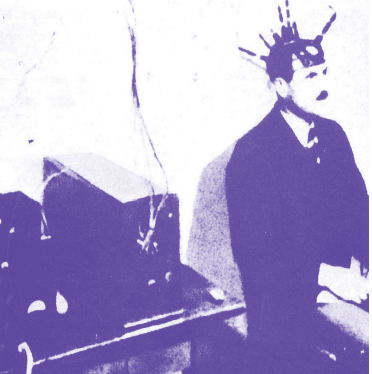
\includegraphics[width=\textwidth]{images/hardware/berger_hardware.png}
        \captionsetup{width=0.9\linewidth}
        \captionsetup{justification=centering}
        \caption{Experimental analog \gls{eeg} recording equipment used by \citet{human_eeg_discovery}.\\Figure by by \citet{oldest_eeg_hardware}.}
        \label{fig:eeg_hardware_evolution_1}
    \end{subfigure}
    \hfill
    \begin{subfigure}{.48\textwidth}
        \centering
        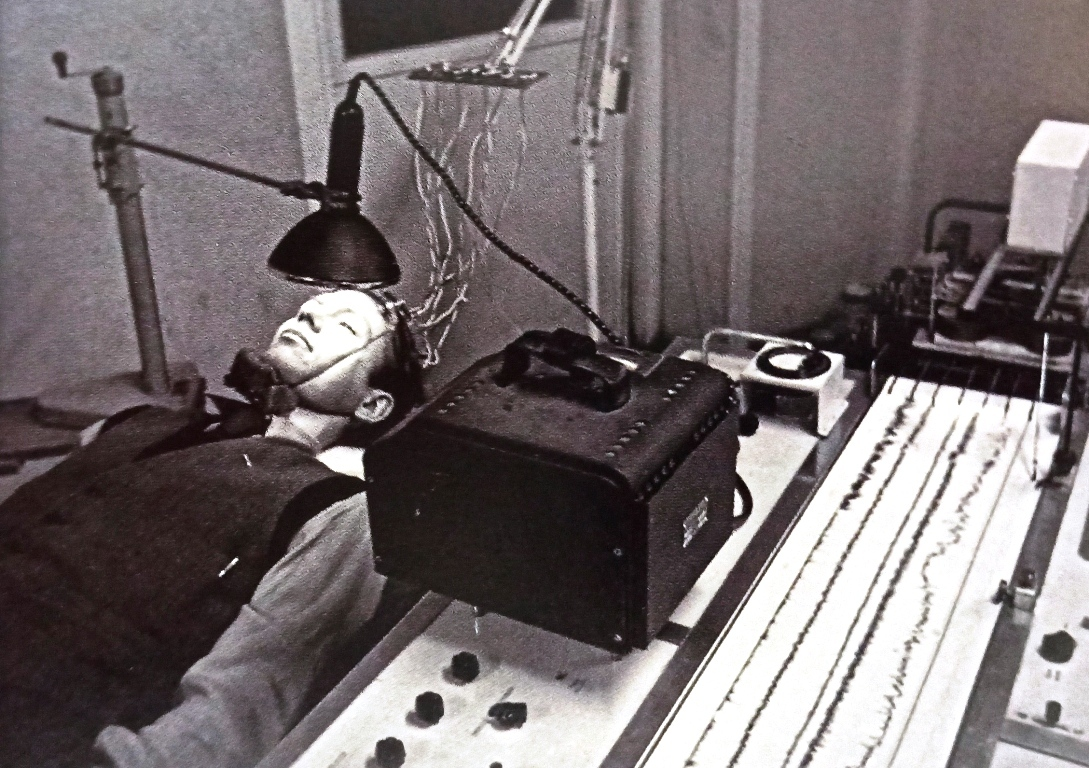
\includegraphics[width=\textwidth]{images/hardware/eeg_1950.jpg}
        \captionsetup{width=0.9\linewidth}
        \captionsetup{justification=centering}
        \caption{Medical-grade analog \gls{eeg} recording equipment estimated to be from the 1950's. \\Figure by Devotor\footnotemark[1].}
        \label{fig:eeg_hardware_evolution_2}
    \end{subfigure}
    \captionsetup{width=0.9\linewidth}
    \bigskip
    \begin{subfigure}{.48\textwidth}
        \centering
        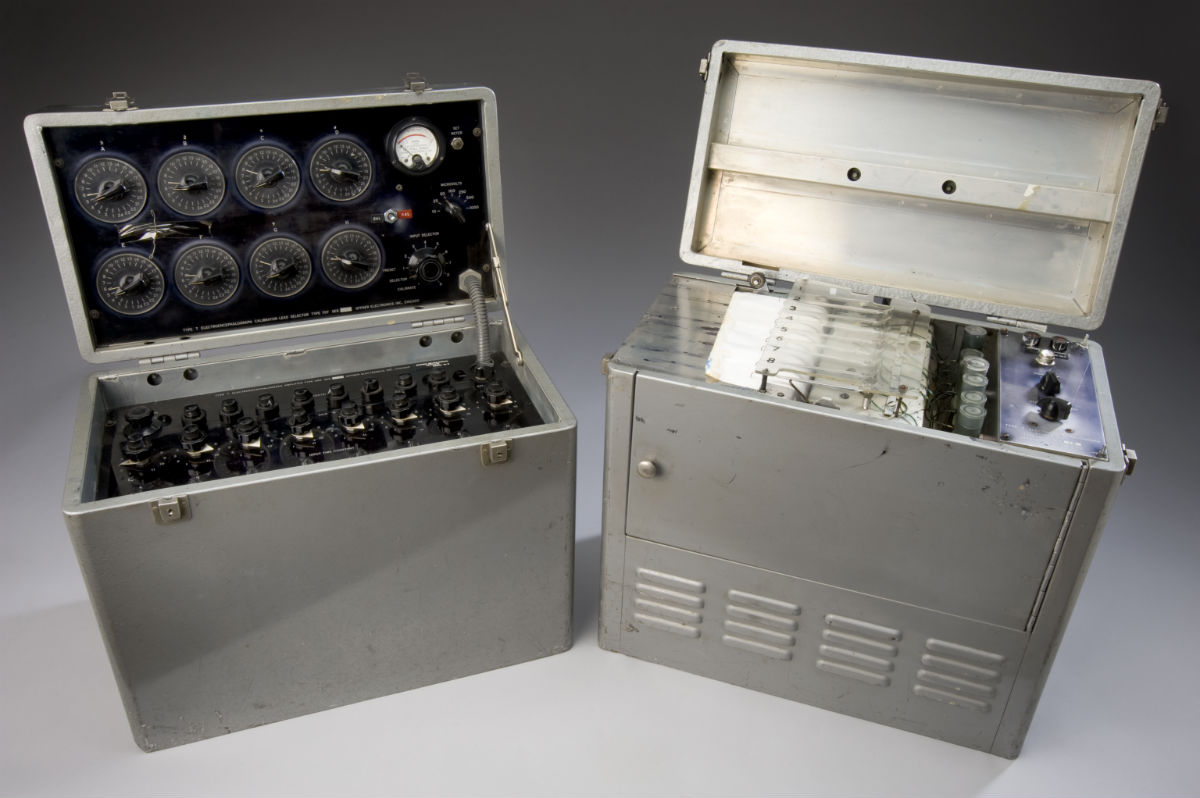
\includegraphics[width=\textwidth]{images/hardware/early_portable_eeg.jpg}
        \captionsetup{width=0.9\linewidth}
        \captionsetup{justification=centering}
        \caption{Early portable analog EEG recording equipment from the late 1950's. \\Figure by Sam Brusco\footnotemark[2]. }
        \label{fig:eeg_hardware_evolution_3}
    \end{subfigure}
    \hfill
    \begin{subfigure}{.48\textwidth}
        \centering
        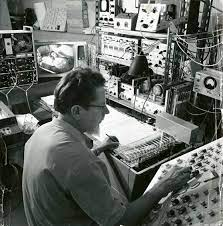
\includegraphics[width=\textwidth]{images/hardware/grey_walter.jpg}
        \captionsetup{width=0.9\linewidth}
        \captionsetup{justification=centering}
        \caption{William Grey Walter and medical-grade analog \gls{eeg} recording equipment, 1964.\\Figure by Burden Neurological Institute\footnotemark[3].}
        \label{fig:eeg_hardware_evolution_4}
    \end{subfigure}
    \captionsetup{width=0.9\linewidth}
    \captionsetup{justification=centering}
    \caption{Early analog \gls{eeg} equipment.}
    \footnotetext[1]{\url{https://www.charismaticplanet.com/the-electroencephalogram-1924/}}
    \footnotetext[2]{\url{https://www.medicaldesignandoutsourcing.com/medtech-memoirs-the-electroencephalograph-eeg/}}
    \footnotetext[3]{\url{http://dx.doi.org/10.15180/181003/019}}
    \label{fig:eeg_hardware_early_analog}
  \end{minipage}  
\end{figure}

% - - - - - - - - - -

\subsection{Usages of invasive systems}
\label{subsec:biomedical_signals_measuring_invasive}

% TODO
\lipsum[1-3]

% - - - - - - - - - -

\subsection{Common EEG artefacts}
\label{subsec:biomedical_signals_measuring_artefacts}

% TODO also discuss how to use them e.g. eye blink as input
\lipsum[1-4]


% ---------------------------------------------- 

\section{Using non-invasive EEG measurements for MI classification}
\label{sec:biomedical_signals_eeg_for_mi_classification}

% TODO
\lipsum[1-2]
% TODO:
%   - XXX
% ----------  
% Questions:
%   - XXX

% In a new chapter, reset the GLS to once again use full version in first occurence
\glsresetall

\chapter{Working with brain-signals}
\label{ch:processing_signals}

% ---------------------------------------------- 

\section{Role of computer scientists in developing BCI systems}
\label{sec:processing_signals_why_cs}

% TODO
\lipsum[1-3]

% ---------------------------------------------- 

\section{Converting raw EEG data to information rich features}
\label{sec:processing_signals_useful_data}
TODO


% - - - - - - - - - -

\subsection{Hardware and software pre-processing}
\label{subsec:processing_signals_useful_data_preproc}
TODO


% - - - - - - - - - -

\subsection{Common EEG based BCI feature extraction methods}
\label{subsec:processing_signals_useful_data_feature}
% The CSP method performs feature extraction based on learned spatial filters.
% https://www.youtube.com/watch?v=zsOULC16USU

TODO


% ---------------------------------------------- 

\section{Different ways of working with the data}
\label{sec:processing_signals_interpreting}
TODO

% - - - - - - - - - -

\subsection{Manually interpreting the signals}
\label{subsec:processing_signals_interpreting_manual}
TODO


% - - - - - - - - - -

\subsection{Computer aided interpretations}
\label{subsec:processing_signals_interpreting_pc_aided}
TODO

% - - - - - - - - - -

\subsection{Fully automated BCI systems}
\label{subsec:processing_signals_interpreting_automated}
TODO

% - - - - - - - - - -

\subsection{Offline and online BCI systems}
\label{subsec:processing_signals_interpreting_offline_online}
TODO

% ---------------------------------------------- 

\section{The role of machine learning}
\label{sec:processing_signals_interpreting_ml}
TODO

% - - - - - - - - - -

\subsection{Classical machine learning approaches}
\label{subsec:processing_signals_interpreting_ml_classic}
TODO

% - - - - - - - - - -

\subsection{Artificial neural networks and deep learning}
\label{subsec:processing_signals_interpreting_ml_ann_dl}
TODO


% ---------------------------------------------- 

\section{Common issues with BCI development}
\label{sec:processing_signals_common_issues}
TODO

% - - - - - - - - - -

\subsection{Explainability and interpretability of models}
\label{subsec:processing_signals_common_issues_exaplainable}

% TOODO
\Gls{dl} often requires significant processing power and time to train, impacting the affordability of \gls{bci} research.
This is especially true when working with many \gls{eeg} sensors and features, and thus a high dimensional setting. 
\Gls{dl} is often also used in a black-box principle.
This means that the trained system lacks explainability and interpretability.
% TODO explain both terms
Recent governmental reports have suggested that laws will be coming in place to require these properties \citep{eu_ai_blackbox_report, explainable_ai_policy}.

% - - - - - - - - - -

\subsection{Lack of data for exhaustive training and testing}
\label{subsec:processing_signals_common_issues_generalisation}
% e.g. only look at a person we also used in training etc
% TODO:
%   - XXX
% ----------  
% Questions:
%   - XXX

% Checkout Fieldtrip toolbox voor laplacian

\chapter{A general BCI pipeline}
\label{ch:bci_pipeline}
TODO

\section{Training the system}
\label{sec:bci_pipeline_training}
TODO


\subsection{Data gathering and windowing}
\label{subsec:bci_pipeline_training_data_gathering_windowing}
TODO


\subsection{Pre-processing}
\label{subsec:bci_pipeline_training_preprocessing}
TODO


\subsection{Feature extraction and generation}
\label{subsec:bci_pipeline_training_features}
TODO


\subsection{Training a ML classification model}
\label{subsec:bci_pipeline_training_classification_model}
TODO

\section{Using the system}
\label{sec:bci_pipeline_using}
TODO


\subsection{Applying the trained classifier}
\label{subsec:bci_pipeline_using_classifier}
TODO


\subsection{Moving towards an online system}
\label{subsec:bci_pipeline_using_going_online}
TODO


% TODO:
%   - XXX
% ----------  
% Questions:
%   - XXX

\chapter{Three signal system for live control}
\label{ch:final_system}
TODO

\section{Overview of the system}
\label{sec:final_system_overview}
TODO


\subsection{TODO}
\label{subsec:final_system_overview_XXX}
TODO


% TODO:
%   - XXX
% ----------  
% Questions:
%   - XXX

\chapter{Using the system and verifying the results}
\label{ch:using_system}
TODO

\section{Performed experiments}
\label{sec:performed_experiments}
TODO


\subsection{TODO}
\label{subsec:performed_experiments_XXX}
TODO


% TODO:
%   - XXX
% ----------  
% Questions:
%   - XXX

\chapter{Self reflection and conclusion}
\label{ch:conclusion}
TODO

\section{Usefulness of the result }
\label{sec:conclusion_usefulness}
TODO


\subsection{TODO}
\label{subsec:conclusion_usefulness_XXX}
TODO




\backmatter%

% Glossary
\glsaddall
\printnoidxglossary[type=\acronymtype,title=List of abbreviations, nonumberlist, style=listgroup]
%\addcontentsline{toc}{chapter}{List of abbreviations}

% References list (show even non cited)
\nocite{*}
\printbibliography[heading=bibintoc, title={References}]
\end{document}













